In this section, we provide the big picture view of the complete Pandora $\nu_e$ analysis, starting from our selection philosophy and ending with our strategy regarding systematics. A deeper dive into each topic is provided in note's following sections. 

\subsection{$\nu_e$ Selection Philosophy \textcolor{green}{David ... (P.R. Elena) }}
\par Several proposals have been made to explain the nature of the MiniBooNE LEE anomaly. It is fair to say that a large amount of uncertainty remains in the community regarding what may have generated such an excess of EM events: this analysis works within the $\nu_e$ excess hypothesis.  To best explore the potential new physics in the $\nu_e$ channel at low energy, this analysis aims to perform an inclusive multi-channel measurement of $\nu_e$ interactions without relying on kinematic variables which depend upon neutrino-interaction models. A multi-channel approach can reduce systematic uncertainties dependent on the chosen interaction model in addition to building stronger confidence against issues with the MC simulation.

\par By performing three different $\nu_e$ selections, we aim to isolate three topologies: the $\nu_e$ inclusive (1$e$X$p$X$\pi$), 1$e$N$p$0$\pi$, and a 1$e$0$p$0$\pi$ channels. A schematic summarizing the strengths and features of each selection is shown in Table~\ref{tab:selectionsNue}. The 1$e$N$p$0$\pi$ and 1$e$0$p$0$\pi$ selections are orthogonal and share a common pre-selection, which splits at the stage in which presence of a final state proton in the event is determined; these two channels combined match the MiniBooNE signal channel (1$e$X$p$0$\pi$). The inclusive $\nu_e$ selection currently is developed independently of the other two selections: therefore, its selected events are not orthogonal to the 1$e$X$p$0$\pi$ pool of candidates.
%\textcolor{red}{Should we add that our main selection is the 1$e$N$p$0$\pi$? }

\begin{comment}
\par We perform three $\nu_e$ selections, each aimed at leveraging particular strengths, and designed with cuts tailored to exploit as much information in a given channel topology as possible. The analysis is comprised of a $\nu_e$ inclusive, a 1$e$N$p$0$\pi$, and a 1$e$0$p$0$\pi$ selection. A schematic summarizing the strengths and features of each selection is shown in table~\ref{tab:selectionsNue}. The 1$e$N$p$0$\pi$ and 1$e$0$p$0$\pi$ selections are orthogonal and share a common pre-selection, which splits at the stage in which presence of a final state proton in the event is determined; these two channels combined match the MiniBooNE signal channel (1$e$X$p$0$\pi$). The inclusive $\nu_e$ selection currently is developed independently of the 1$e$N$p$ selection and therefore its selected events are not independent.
\end{comment}



%\begin{figure}[ht]
%\begin{center}
%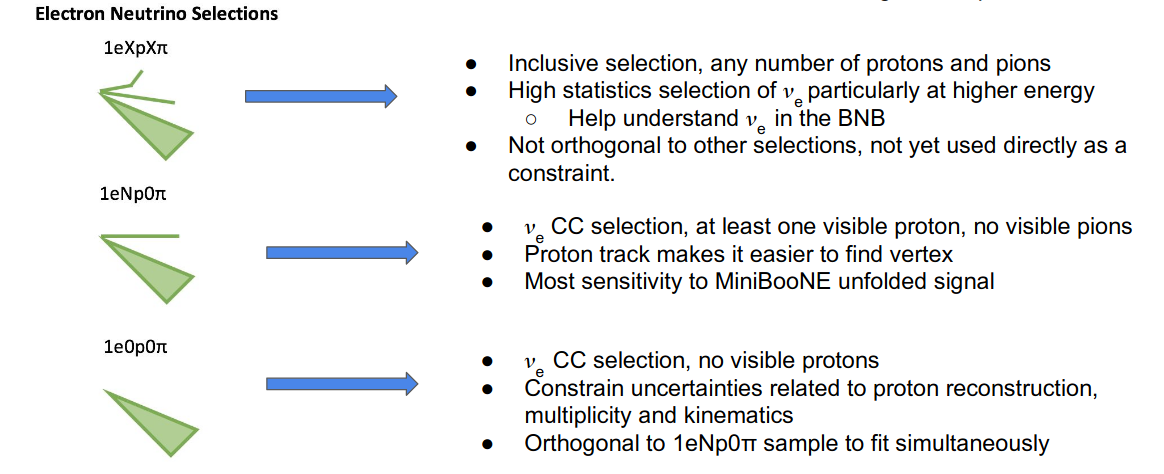
\includegraphics[width=0.85\textwidth]{introduction/nueselections.png}
%\caption{\label{fig:nueselections}Schematic of the three $\nu_e$ selection in this analysis, outlining the goals and strengths of each. In this work, the threshold for a visible proton at truth-level proton is 40 MeV of KE. $N$ refers to one or more and $X$ to any number of final state particles of a given category.}
%\end{center}
%\end{figure}


\begin{table}[ht]
\caption{\label{tab:selectionsNue} Schematic of the three $\nu_e$ selections, outlining the definition and goals of each. In this work, the threshold for a visible proton at truth-level proton is 40 MeV of KE. N refers to one or more and X to any number of final state particles of a given category.}
\centering
\begin{tabular}{ m{0.1\textwidth} | m{0.2\textwidth}  m{0.45\textwidth}  }
Channel & Description & Goal \\
\hline
 \begin{center}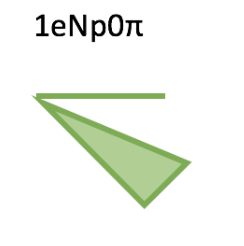
\includegraphics[width=0.1\textwidth]{introduction/1eNp}\end{center}& At least one visible proton and no visible pions & Most sensitive channel to MiniBooNE unfolded signal. The presence of a proton facilitates vertex finding.\\
\hline
 \begin{center}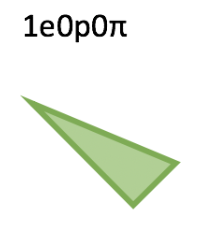
\includegraphics[width=0.1\textwidth]{introduction/1e0p}\end{center}& No visible protons and no visible pions & Constrain uncertainty related to proton reconstruction, multiplicity and kinematics for the 1$e$N$p$0$\pi$ channel.\\
\hline
\begin{center}\includegraphics[width=0.1\textwidth]{introduction/inclusive} \end{center} & Inclusive Selection: any number of protons and pions & Helpful to understand $\nu_e$ in the BNB: high statistic selection, especially at higher energies ($>$ 700 MeV). Not used as a constraint for other channels. \\
\hline
\end{tabular}
\label{tab:gt}
\end{table}


\par %\textbf{agnostic selection} 
In devising the selections presented above, we have deliberately chosen to not rely on cuts that make use of kinematic features of low-energy $\nu_e$ events. This allows the analysis to be agnostic to possible sources of new physics, and limits model dependence associated with assumptions on intrinsic $\nu_e$ interaction kinematics. Furthermore, an agnostic selection strategy allows to explore the kinematics of $\nu_e$ candidate events after their selection, for a full investigation of the origin of a potential anomaly. Implementing this choice requires the ability to fully leverage the information provided by the MicroBooNE LArTPC for $\nu_{\mu}-\nu_e$ and $e-\gamma$ separation. Significant progress has been made in developing tools for this goal, and will be described in subsequent sections. 




\subsection{Signal Model \textcolor{green}{David  ... (P.R. Elena) }}
\begin{comment}
%%%%%%% these are various parts that have been moved/modified
In order to benchmark the performance of the analysis it is valuable to have a signal model which can be used to assess the analysis' sensitivity.  This section describes the choice of model used for this purpose. It is important to stress that the signal model used serves the purpose of benchmarking the analysis' sensitivity, but the ultimate goal of our analysis remains to measure the rate of $\nu_e$ interactions in the BNB and report whether the observation is consistent or not with MicroBooNE's MC prediction.

\par Ultimately many signal models can be produced to test an analysis' sensitivity, each with its own set of important assumptions and caveats. % Or...
Ultimately any signal model used to test the analysis' sensitivity will carry a set of important assumptions and caveats. 
While reporting sensitivities for the MB-$\nu_e$ LEE model is useful, it is not exhaustive in being able to address MicroBooNE's ability to address MiniBooNE's anomaly. 
\end{comment}


\par  Many models can be devised to explain the MiniBooNE LEE as an excess of $\nu_e$ interactions, each model relying on a given (new) physics production mechanism and set of assumptions on the detector response. This section describes the signal model chosen by the collaboration to benchmark the sensitivity of all $\nu_e$ LEE analyses, including ours.  While a signal model is a useful tool, it is important to stress that any signal model carries a set of important assumptions and caveats, and that the ultimate goal of our analysis remains to measure the rate of $\nu_e$ interactions in the BNB, reporting whether the observation is consistent or not with MicroBooNE's MC prediction. Answering whether MicroBooNE's observation is consistent with the MiniBooNE LEE anomaly is beyond the scope of this work, and something not achievable without significant work for both MiniBooNE and MicroBooNE.
\begin{comment}
\par To test this analysis' sensitivity, a model explaining the MiniBooNE LEE  as an excess of $\nu_e$ interactions must be produced and used to generate simulated events in MicroBooNE. Many such models can be devised, each relying on a given (new) physics production mechanism and set of assumptions on detector response. 
\end{comment}

\par  The signal model used to generate simulated events in MicroBooNE and to compute the primary sensitivity quoted by this analysis  is the MiniBooNE-unfolded LEE model, referred to as \textbf{MB-$\nu_e$ LEE} model \cite{C,C2}. In this model, all excess LEE events are assumed to be due to $\nu_e$ interactions with a value of true energy obtained by unfolding from the reconstructed CCQE energy of MiniBooNE LEE events, as recorded by MiniBooNE's data. This procedure is performed by relying on MiniBooNE's energy smearing matrix. The resulting true neutrino energy distribution is shown in figure~\ref{fig:minibooneunfolded}. There are several limitations to this model worth observing, some technical, others conceptual. On a technical level, the model is composed of a binned event distribution, rather then a parametrized or analytic prediction of the expected $\nu_e$ spectrum. Additionally, no events below 200 MeV of true energy exist in this model. 
\begin{figure}[ht]
\begin{center}
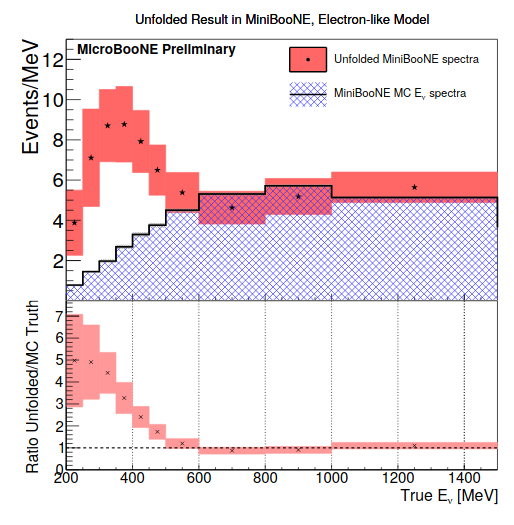
\includegraphics[width=0.45\textwidth]{introduction/unfoldedminiboone.png}
\caption{\label{fig:minibooneunfolded}MB-$\nu_e$ LEE signal model extracted from MiniBooNE's results.}
\end{center}
\end{figure}
Conceptual issues can be raised in association with the various assumptions made to generate the model. These include the strong reliance on MiniBooNE's simulation in order to unfold reconstructed to true neutrino energy, and the choice of such an unfolding procedure (performed as a function of $E_{\rm CCQE}$ rather then EM energy and $\theta$, for example).
It is especially important to note that the chosen model strongly favors the interpretation of MiniBooNE events as originating from very low energies (200-400 MeV) for which achieving high sensitivity may come at the cost of omitting a robust analysis at higher energies. This is something the analysis tries to avoid by developing an inclusive and kinematically unbiased analysis workflow. At the same time, we explore additional models for sensitivity calculations, most notably a 3+1 sterile-neutrino oscillation model. This is discussed in more detail in section~\ref{sec:Sensitivity2Osc}.
\par Figure~\ref{fig:nuerate} shows the expected $\nu_e$ rate as a function of true neutrino energy split by final-state topology for the available MicroBooNE dataset of $10.1E20$ POT. % with a 10 cm FV. 
 MB-$\nu_e$ LEE signal events are shown in orange.
\begin{figure}[H] 
\begin{center}
    \begin{subfigure}[b]{0.45\textwidth}
    \centering
    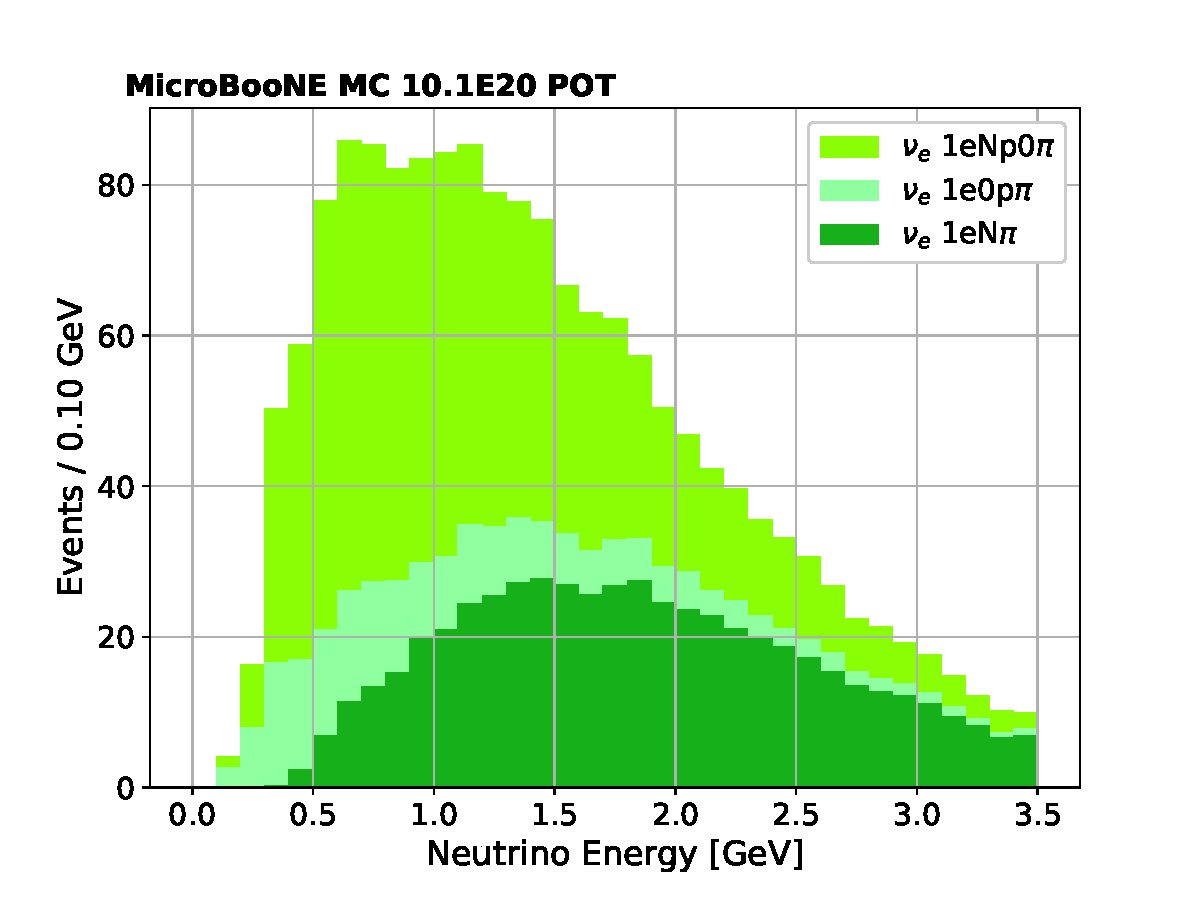
\includegraphics[width=1.00\textwidth]{introduction/nue_rate_MCC9.pdf}
    %\caption{\label{fig:nuerate:prediction}}
    \end{subfigure}
    \begin{subfigure}[b]{0.45\textwidth}
    \centering
    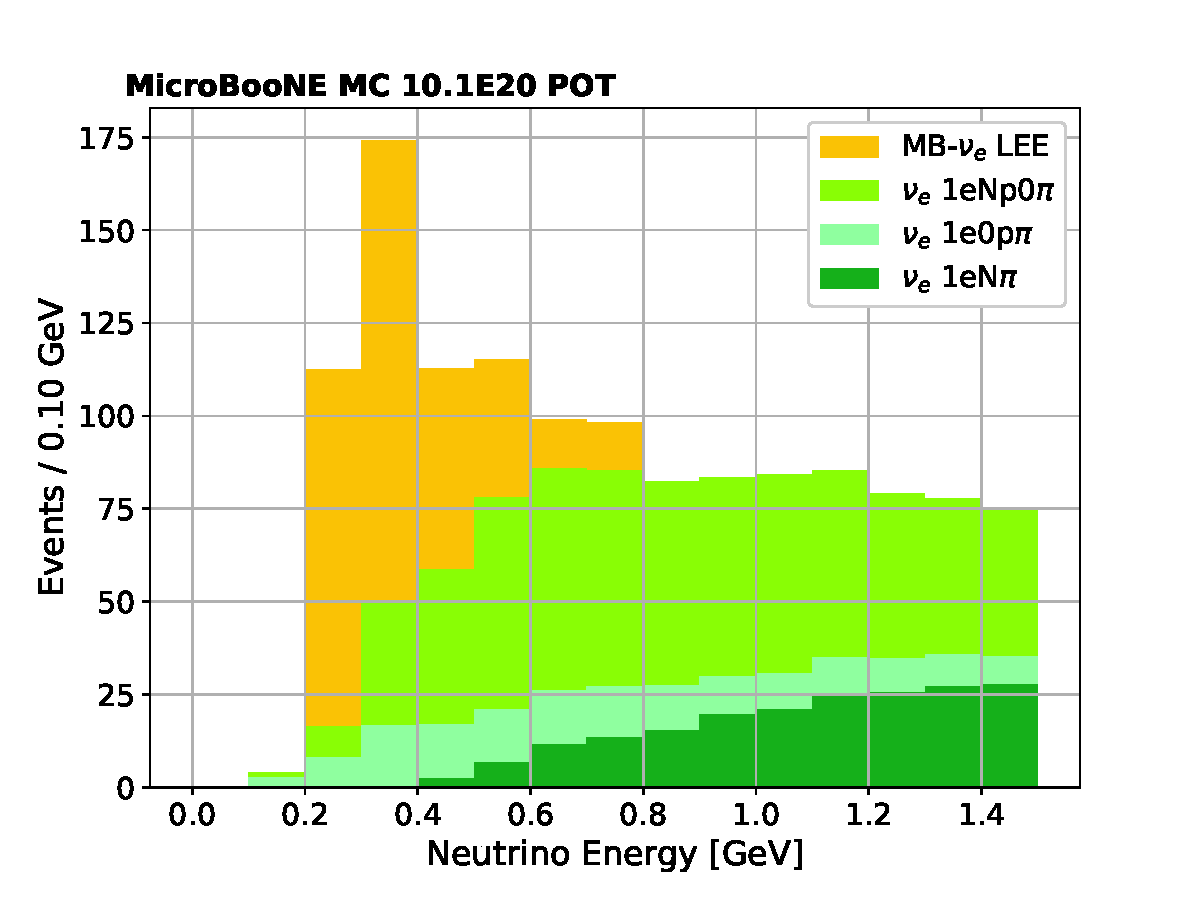
\includegraphics[width=1.00\textwidth]{introduction/nue_rate_MCC9_LEE.pdf}
    %\caption{\label{fig:nuerate:prediction:MC}}
    \end{subfigure}
\caption{\label{fig:nuerate}Expected $\nu_e$ rate in MicroBooNE for $10.1E20$ POT %in a 10-cm FV 
 subdivided by event topology (1$e$N$\pi$,1$e$N$p$0$\pi$, and 1$e$N$p$0$\pi$). The right-hand side figure highlights the low energy region with the unfolded $MB-\nu_e$ LEE signal prediction in orange.}
\end{center}
\end{figure}

\subsection{Goals of the $\nu_{\mu}$ Selection \textcolor{green}{David   ... (P.R. Elena)}}
\label{ssec:goalsofnumusel}
\begin{comment}
\par For the purpose of this analysis, measurements of $\nu_{\mu}$ interactions are aimed at reducing modeling uncertainties for intrinsic $\nu_e$ events and backgrounds, with the goal of reducing systematic uncertainties in order to be able to claim the observation of new physics were a measurement of $\nu_e$ interactions differ significantly from the expected intrinsic rate. This section describes why such a data-driven constraint is needed and what are the choices which motivate the approach taken in this analysis.
\end{comment}
\par In the context of this analysis, measurements of $\nu_{\mu}$ interactions are aimed at reducing modeling uncertainties for intrinsic $\nu_e$ events and backgrounds. Event reconstruction and $\nu_e$ identification are only one of the challenges in this analysis:  in order to make statements on whether the observed $\nu_e$ rate indicates the presence of new physics, a well understood prediction of the intrinsic $\nu_e$ rate is needed. 

\par Uncertainties in the expected $\nu_e$ rate are associated to reconstruction efficiencies (detector effects) as well as modeling uncertainties in both the $\nu_e$ flux  and neutrino-argon cross-section predictions. Here, we focus on describing the strategy to deal with the latter. In the case of a single detector experiment, %uncertainties in the intrinsic $\nu_e$ interaction rate are rather large:  and can limit the ability to associate a $\nu_e$ measurement with potential new physics if not a constraint through additional measurements is needed. 
flux uncertainties for $\nu_e$ calculated from the beam simulation are $\mathcal{O}$(10\%) above 800 MeV and grow to 40\% at 200 MeV;  cross-section uncertainties are also large, due to the scarcity of $\nu$-Ar cross-sections measurements -- especially at low energy -- and due to the complex modeling of neutrino interactions on heavy targets such as argon. Combining all effects, the uncertainty on the $\nu_e$ interaction rate in the few-hundred MeV energy range in MicroBooNE could be as high as 100\%.
\par To reduce modeling uncertainties on the expected rate of $\nu_e$ interactions, data-driven constraints are required. These can be performed through measurements of $\nu_{\mu}$ interactions impacted by the same underlying modeling uncertainties. In order to constrain flux uncertainties, we rely on the fact that $\nu_e$ and $\nu_{\mu}$ intrinsic to the beam are produced by the decay of the same parent $\pi$ and $K$ flux. Similarly, we rely on the charged-current interaction mode $\nu_{l} + Ar \rightarrow l + X$ common to both $\nu_{\mu}$ and $\nu_e$ interactions to constrain the uncertainties on the $\nu_e$ interaction modeling.


\begin{comment}

The complexity of $\nu$-Ar interactions and of hadronic interactions in the beamline mean that many different handles and measurements of $\nu_{\mu}$ interactions can play a role in constraining different uncertainties. As examples, measurement of CC and NC $\pi^0$ production constrain resonant interactions and thus $\pi^0$ backgrounds to the $\nu_e$ selection, and measurements of high-energy $\nu_{\mu}$ interactions can help constrain the kaon flux in the beam, which contributes substantially to the production of intrinsic $\nu_e$s. Likewise, measurements of low-energy $\nu_{\mu}$s can help constrain poorly understood $\nu$-Ar interaction models in the few-hundred MeV energy regime, a critical requirement for this analysis. The neutrino identification work developed for this analysis, referred to as \texttt{SliceID} and described in section~\ref{sec:sliceID}, is a highly efficient and topology agnostic selection that enables a vast program of $\nu_{\mu}$ measurements, allowing for flexibility in selecting topologies that may have the strongest constraining power and thus most benefit the $\nu_e$ analysis. At the current time, as described in the remainder of this section and in section~\ref{sec:systematics}, the emphasis is on the measurement of low-energy $\nu_{\mu}$ interactions with the goal of constraining the large uncertainties in low-energy $\nu_e$ events which significantly impact the analysis.
\par To further motivate the need for low energy $\nu_{\mu}$ interactions, we describe two important ways in which such a dataset can benefit the reduction of modeling uncertainties for $\nu_e$ interactions.
\end{comment}
\par The richness of $\nu$-Ar interactions and of hadronic interactions in the beamline offers a number of different handles 
to constraint different uncertainties via the measurements of $\nu_{\mu}$ interactions.
As examples, measurements of CC and NC $\pi^0$ production can be used to constrain resonant interactions and thus $\pi^0$ backgrounds to the $\nu_e$ selection;  measurements of high-energy $\nu_{\mu}$ interactions can help constrain the kaon flux in the beam, which contributes substantially to the production of intrinsic $\nu_e$s. Likewise, measurements of low-energy $\nu_{\mu}$s can help constrain poorly understood $\nu$-Ar interaction models in the few-hundred MeV energy regime, a critical requirement for this analysis.  At the current time, we focus our effort on the study with the bigger impact to the analysis: we perform the measurement of low-energy $\nu_{\mu}$ interactions with the goal of constraining the large uncertainties in low-energy $\nu_e$. A detailed  description of this constraint is shown in the remainder of this section and in section~\ref{sec:systematics}.
%At the current time, our effort is focused on the measurement of low-energy $\nu_{\mu}$ interactions with the goal of constraining the large uncertainties in low-energy $\nu_e$ events which significantly impact the analysis; a detailed  description of this constraint is shown in the remainder of this section and in section~\ref{sec:systematics}.
 However, it should be noted that the neutrino identification work described in section~\ref{sec:sliceID} results in a highly efficient and topology agnostic selection: such a flexible selection allows for a number of $\nu_{\mu}$ measurements and their associated constraints to be implemented in case the $\nu_e$ analysis needs a stronger constraining power. 



\par To further motivate the need to study low energy $\nu_{\mu}$ interactions, we describe two important ways in which such a dataset can lead to a reduction of modeling uncertainties for $\nu_e$ interactions. Figure~\ref{fig:numuconstraint:flux} shows the flux correlation for $\nu_{\mu}$ (bottom left) and $\nu_e$ (top right) interactions obtained from MicroBooNE's adaptation of the BNB flux simulation developed by MiniBooNE~\cite{bib:fluxmcc9,bib:fluxtechnote}. Red (blue) areas show large (anti-)correlation. The top-left or bottom-right quadrants show the strength of correlations between the two flavors. For $\nu_e$ energies below 1 GeV, correlations are strongest with $\nu_{\mu}$ interactions at low energy \textcolor{blue}{should we add some more details on the assumptions behind this correlation matrix? or on how this correlation matrix is calculated (is it simply from the beam MC?) Elena}. Figure~\ref{fig:numuconstraint:xsec} shows different cross-section predictions for $\nu_{\mu}$ and $\nu_e$ interactions. The dashed and solid curves represent the CCQE cross-section used in MCC8 vs. MCC9 respectively. Below 400 MeV, the difference in event rates for different models is larger then 100\%. The large differences between these curves, particularly at low energy, indicate the strong need to constrain cross-section uncertainties with MicroBooNE's own data. 
\begin{figure}[ht] 
\begin{center}
    \begin{subfigure}[b]{0.42\textwidth}
    \centering
    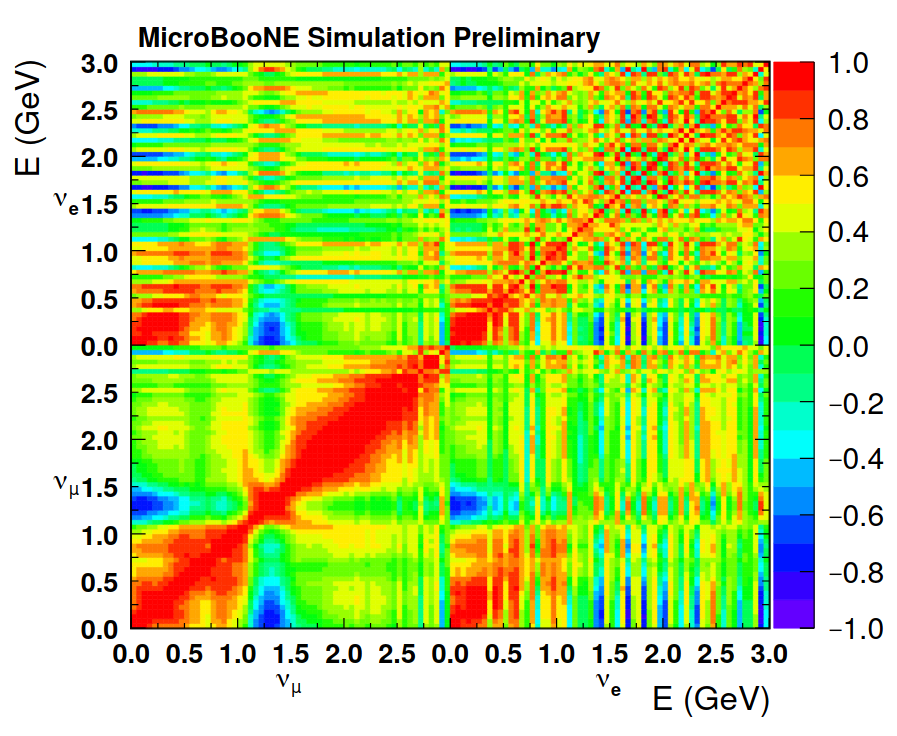
\includegraphics[width=1.00\textwidth]{introduction/fluxcorrelation.png}
    \caption{\label{fig:numuconstraint:flux}}
    \end{subfigure}
    \begin{subfigure}[b]{0.3\textwidth}
    \centering
    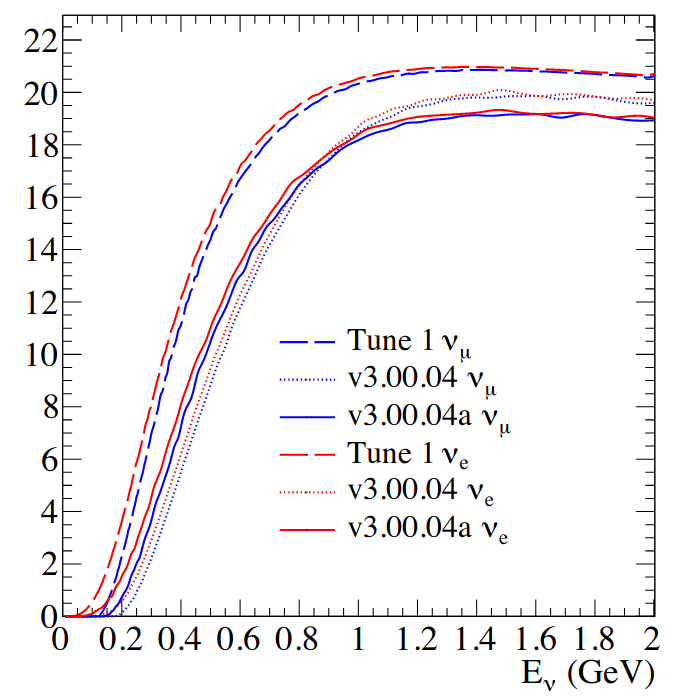
\includegraphics[width=1.00\textwidth]{introduction/xsec_mcc8_mcc9.png}
    \caption{\label{fig:numuconstraint:xsec}}
    \end{subfigure}
\caption{\label{fig:numuconstraint} (a) $\nu_{\mu}$-$\nu_e$flux correlation matrix. (b) Different cross section models for CC interactions \textcolor{blue}{Y axis label is missing}.  }
\end{center}
\end{figure}

\subsection{Systematics \textcolor{green}{David... (P.R. Elena)}}
\par This section gives a brief overview of how detector and modeling uncertainties are accounted for in the analysis. The estimation of systematics is performed in section~\ref{sec:systematics}.
\par \noindent \textbf{Detector Systematics}: Detector modeling in MicroBooNE has undergone significant updates in the past year, in part as a result of the large impact that detector systematics have had on 2018 analyses \cite{bib:CCpi0, bib:CCincl}. Detector effects with significant impact on the analysis can be broken up into three main categories:
\begin{itemize}
    \item[-] Wire-Response modeling: the response of MicroBooNE's electronics to drifting charge is a complex subject described in three past publications~\cite{bib:noise,bib:SP1,bib:SP2}. The work of these papers in improving the understanding and modeling of noise and field-response effects has been implemented in the current detector simulation and is expected to lead to a reduction in what for MCC8 analysis comprised the largest detector uncertainty.
    \item[-] Space-Charge modeling: MicroBooNE's space-charge model has changed significantly since 2018, moving from a calculation-based~\cite{bib:SCEsim} implementation of electric field distortions to a data-driven E-field map~\cite{bib:SCEdata} implemented in simulation and reconstruction. Due to the large position distortions (and, though smaller, charge distortions) SCE can significantly impact an analysis through the determination  of fiducial boundaries, tracking and energy resolution.
    \item[-] Scintillation light modeling: MicroBooNE's model of scintillation light production has not changed significantly since the beginning of data-taking, and has known limitations. Of particular importance to this analysis, which aims to use a dataset spanning four years, is the known and significant time-dependent variation of MicroBooNE's light response. This analysis takes several steps to correct for, and mitigate the impact of light mismodeling. Triggering on low-energy signal $\nu_e$ events, and cosmic-rejection are particularly sensitive to scintillation light detector effects.
\end{itemize}
\emph{An additional detector effects that needs to be accounted for is ion Recombination which impacts the detector's calorimetric response. Tailored studies and proton samples are being developed to assess ion recombination modeling accuracy in MCC9 but are not available at the time of writing of this note.}
\par \noindent \textbf{Flux and Cross-Section Modeling} Uncertainties in flux and cross-section modeling are treated through a \emph{multi-sim} approach, where underlying parameters that are input to the modeling are varied in a correlated way. Flux uncertainties are taken from the MiniBooNE BNB flux simulation adapted to MicroBooNE~\cite{bib:fluxmcc9,bib:fluxtechnote}, while $\nu$ interaction uncertainties are handled within the \texttt{GENIE} reweighting package, as described in~\cite{bib:geniesupportnote}. \emph{We note that the \texttt{GENIE} event reweighting infrastructure is still in development and likely to be updated or further expanded on in the future. Finally, uncertainties associated with pion and proton re-interactions in argon were unavailable when this version of the Tech Note was produced and not included at this stage.} 

\subsection{Sensitivity Estimation \textcolor{green}{Nico/Maya... (P.R Elena)}}
In order to extract information from the selected events, a simple hypothesis test is performed.
Given an observable quantity, such as a measurement of the energy deposited by the neutrino interaction, the hypothesis in which the observed spectrum of events is entirely due to the standard model, $H_0$, is tested against an alternative hypothesis $H_1$.
The alternative hypothesis $H_1$ consists of all the known background plus the LEE unfolded signal from MiniBooNE (MB-$\nu_e$ LEE), though an oscillation signal has also been studied, as shown in section \ref{sec:Sensitivity2Osc}.
For the MB-$\nu_e$ LEE signal, the hypothesis test is simple in that the comparison of two different hypotheses is performed and no parameter is inferred from the data.

%The hypothesis test is simple in the sense no parameter is fitted from the data, but we limit ourselves to a comparison of two different hypotheses.

A test statistic is chosen in order to condensate all information of the observables in one number.
Through toy experiments, the expected distributions of the test statistic under the two hypotheses is calculated; the separation power is computed by taking the median p-value with respect to $H_0$ under the assumption that %one might observe if 
 $H_1$ is true. This is the discovery sensitivity, i.e. the sensitivity to reject $H_0$ when $H_1$ is true.
We studied the sensitivity in different cases. First, we describe in detail the sensitivity calculation considering only statistical uncertainties. Given that only a handful of events pass the exclusive selections, the impact of statistical uncertainties plays a large role in determining the analysis' ultimate sensitivity. We also include systematic uncertainties using the covariance matrix formalism and the SBNfit package, as described in section \ref{subsec:sensitivity_syst_uncertainty}.
Finally, the observed spectra from the \nueccnopinp and the \numu selections are analyzed simultaneously using a single covariance matrix to constraint the systematic uncertainties and thus increase the sensitivity.

\subsection{Analysis Status \textcolor{red}{Elena/David/ Group discussion}}

\par The work presented in this note has matured into a robust and comprehensive analysis, with strong tools which are able to leverage the calorimetric and topological imaging of the LArTPC technology to identify in a kinematically agnosic selection $\nu_e$ interactions in MicroBooNE's BNB dataset. The analysis, as it stands, is able to make interesting conclusions on the $\nu_e$ content of the BNB flux, with the primary limitation to the power of these conclusions driven by the low selection efficiency at low energy .
\par Multiple selections have been developed as part of this analysis, all showing generally good data-simulation agreement, as shown in figure~\ref{fig:datamccomparisons} for the \npsel pre-selection (figure~\ref{fig:datamccomparisons:nuepresel}, Run 1) and for the full $\nu_{\mu}$ contained selection (figure~\ref{fig:datamccomparisons:numu}, Run 3).

\begin{figure}[ht] 
\begin{center}
    \begin{subfigure}[b]{0.4\textwidth}
    \centering
    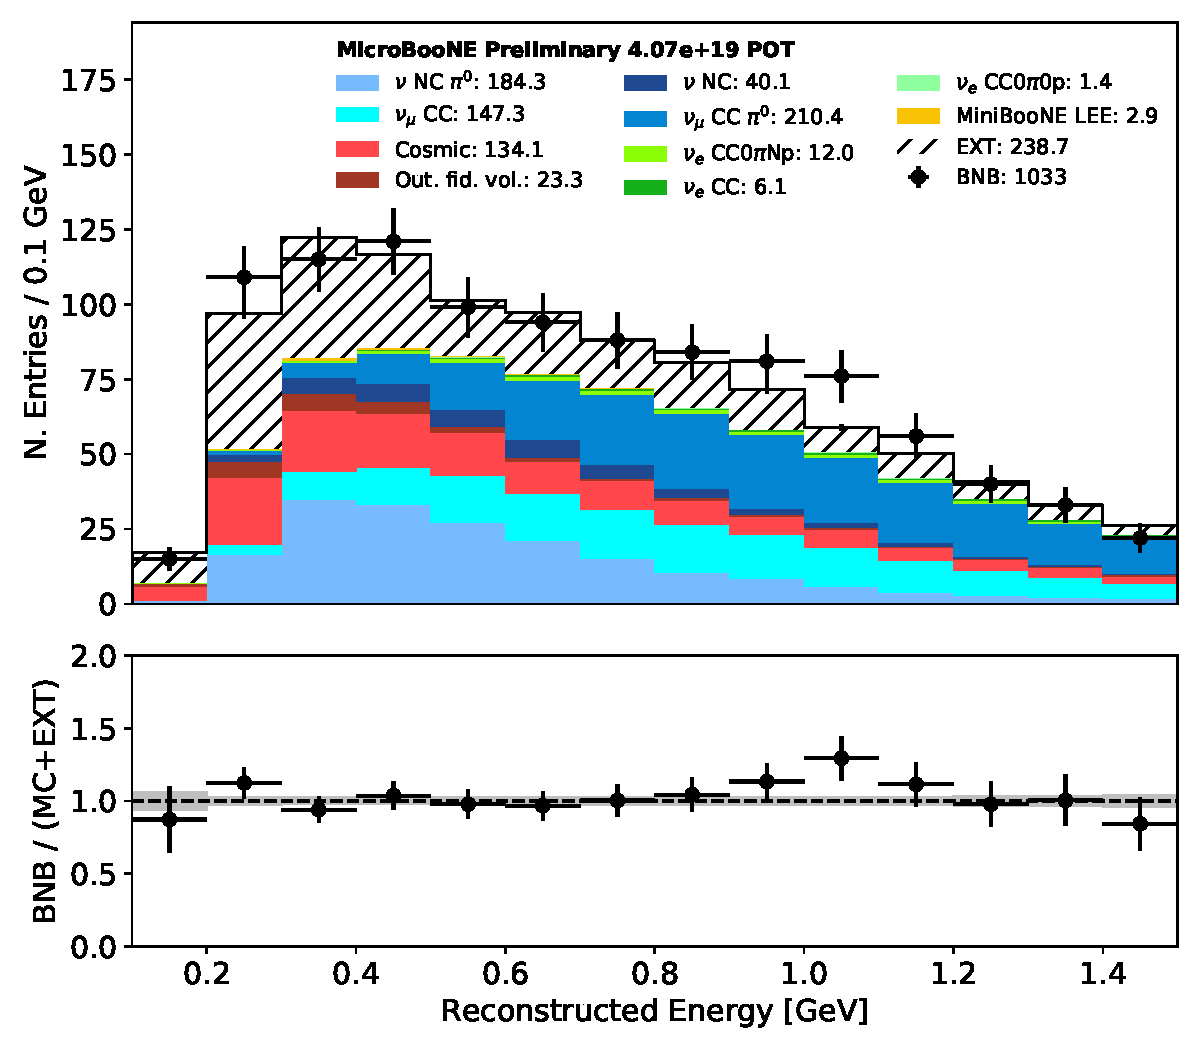
\includegraphics[width=1.00\textwidth]{1eNp/reco_e_01162020_RUN1.pdf}
    \caption{\label{fig:datamccomparisons:nuepresel} \npsel pre-selection for Run  1}
    \end{subfigure}
    \begin{subfigure}[b]{0.44\textwidth}
    \centering
    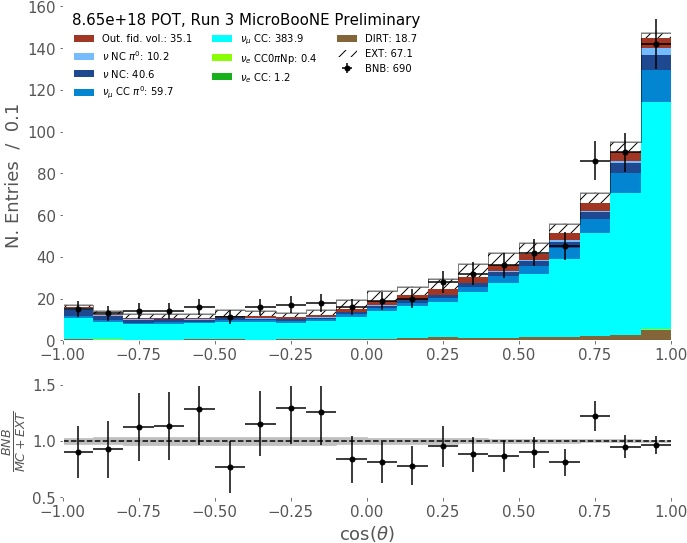
\includegraphics[width=1.00\textwidth]{NuMuCCsel/Images/Ryan/Run3_costheta_withCRT.jpg}
    \caption{\label{fig:datamccomparisons:numu} high-purity $\nu_{\mu}$ for Run 3}
    \end{subfigure}
\caption{\label{fig:datamccomparisons} }
\end{center}
\end{figure}

\par The three $\nu_e$ selections developed in this work all provide strong input to the analysis. Figure~\ref{fig:intro:nueselections} shows the status of the box-cut \npsel (figure~\ref{fig:intro:nueselections:1eNp}), the BDT-based \zpsel selection (figure~\ref{fig:intro:nueselections:1e0p}), and the BDT-based $\nu_e$ inclusive (figure~\ref{fig:intro:nueselections:inclusive}). \par The inclusive channel provides the analysis a tool with which to study the modeling of $\nu_e$ interactions, especially at higher energies, and provides a first validation even with the small dataset currently available. Moving forward, we are exploring ways to use this channel to quantitatively constrain high-energy $\nu_e$ modeling uncertainties.
\par The 1$e$0$p$0$\pi$ channel obtains a purity of 49\% and, even though it currently primarily is sensitive to higher-energy $\nu_e$ interactions, provides a valuable validation of detector and modeling effects which can cause migration from the N$p$ to 0$p$ channel. A quantitative estimation of the impact of this channel is being performed.
\par The \npsel channel, in the box-cut selection, achieves a $5-10$\% efficiency with a 73\%  purity for the cut-based  and a $5-15$\% efficiency with a 81\%  purity for the BDT-based selection. These selections lead to $\mathcal{O}$(10) expected MB-$\nu_e$ LEE signal events and $40-70$ intrinsic $\nu_e$ events for the full Run $1-4$ dataset. The final reconstructed energy distribution for the box-cut selection is shown in figure~\ref{fig:intro:nueselections:1eNp}. The box-cut selection's statistics-only sensitivity is $2.1-2.3\sigma$, depending on the test-statistic used. The low statistics of the predicted signals lead to significant fluctuations in the expected sensitivity, covering the range $1.5-3.1\sigma$. 
 \emph{Given the efficiency and purity obtained with the BDT-based workflow, we expect a higher sensitivity compared to the cut-based workflow.  We are in the process of re-evaluating the BDT-based performance which will be reported in this note after higher statistics MC samples have been included, and a re-calibration of the calorimetry has been completed.} 

\begin{figure}[ht] 
\begin{center}
    \begin{subfigure}[b]{0.28\textwidth}
    \centering
    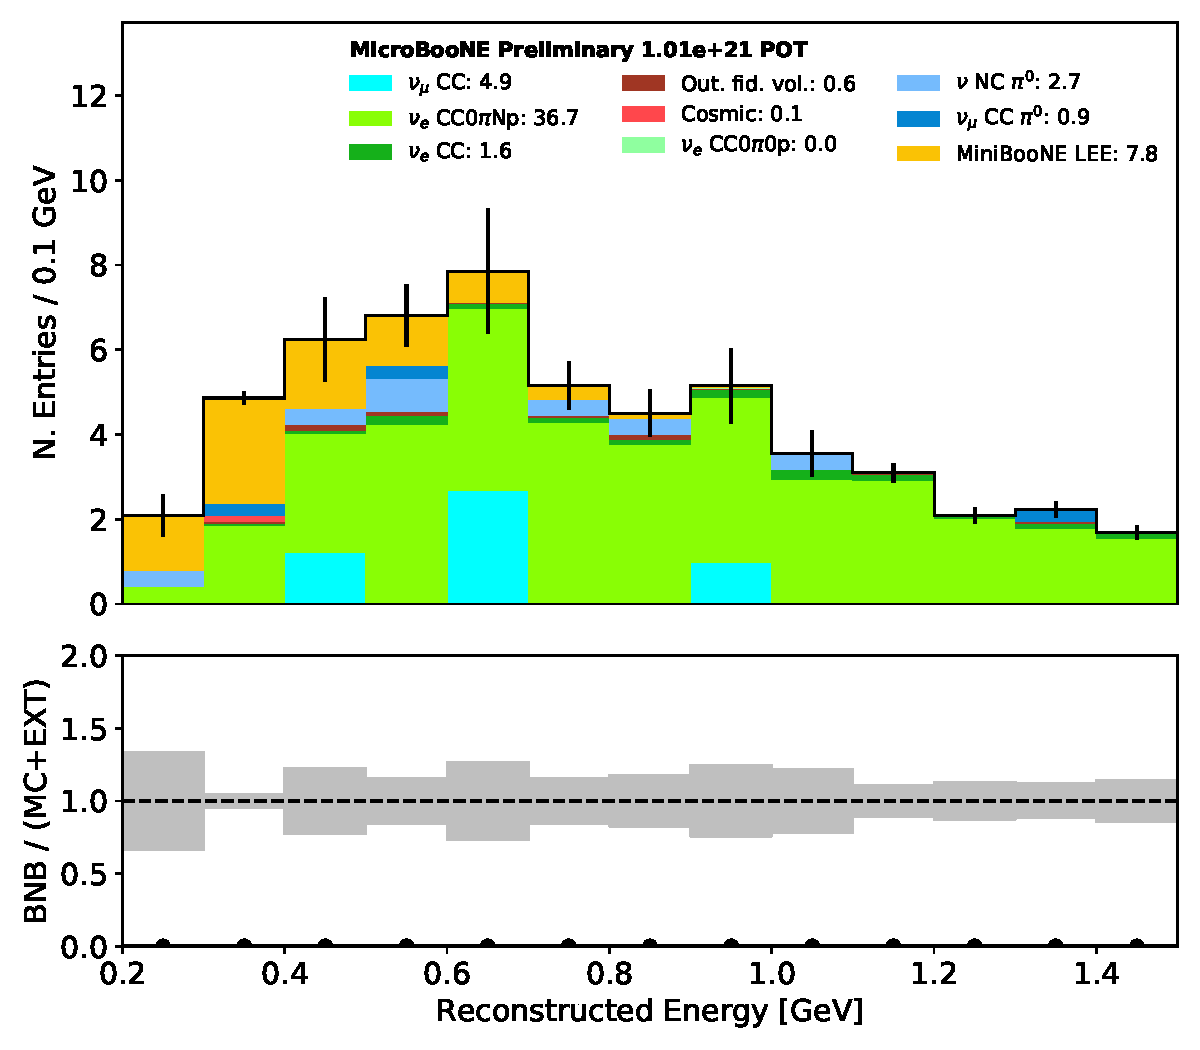
\includegraphics[width=1.00\textwidth]{1eNp/reco_e_01162020_box_RUN1.pdf}
    \caption{\label{fig:intro:nueselections:1eNp} box-cut $\nu_e$ 1$e$0$p$}
    \end{subfigure}
    \begin{subfigure}[b]{0.28\textwidth}
    \centering
    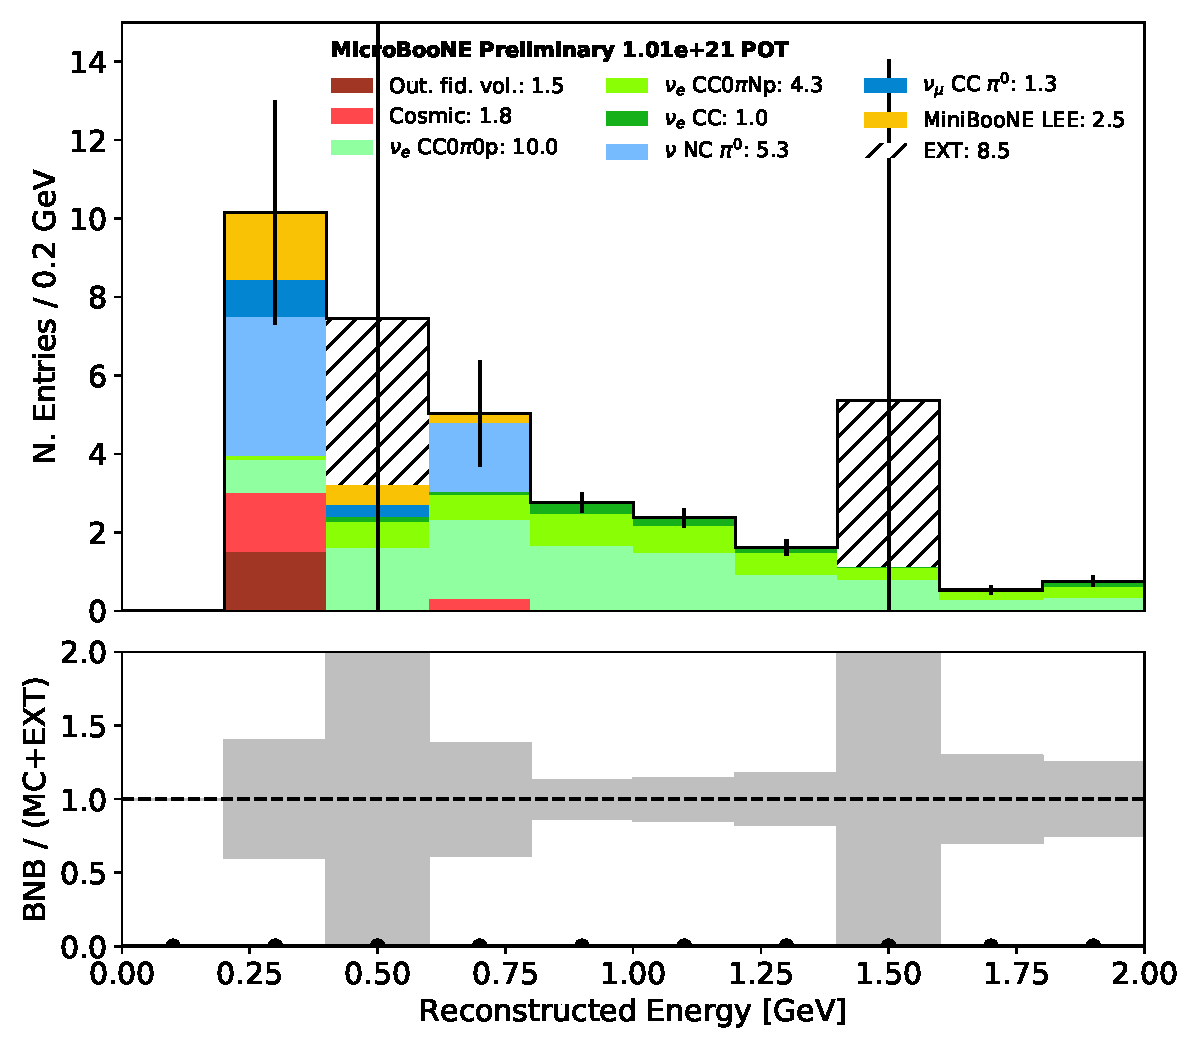
\includegraphics[width=1.00\textwidth]{1e0p/reco_e_01162020_RUN3_bgbdt.pdf}
    \caption{\label{fig:intro:nueselections:1e0p} bdt-based $\nu_e$ 1$e$0$p$}
    \end{subfigure}
    \begin{subfigure}[b]{0.31\textwidth}
    \centering
    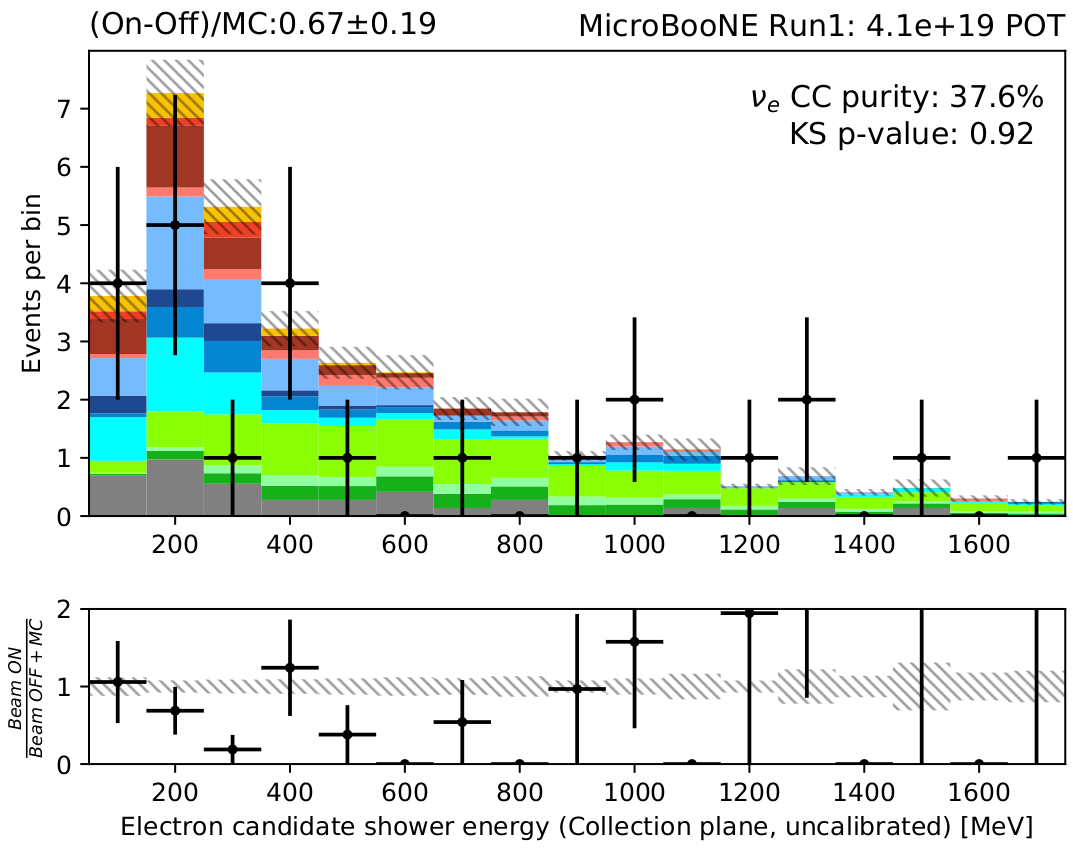
\includegraphics[width=1.00\textwidth]{introduction/nueinclusive.png}
    \caption{\label{fig:intro:nueselections:inclusive} BDT-based $\nu_e$ inclusive}
    \end{subfigure}
\caption{\label{fig:intro:nueselections} }
\end{center}
\end{figure}


\par A particular strength of this analysis consists in the multiple sideband channels available to validate the simulation, reconstruction, and help constrain $\nu_e$ interaction uncertainties. A high statistics $\pi^0$ sideband (section~\ref{sec:controls:pi0}) provides confidence in the performance of the analysis' shower reconstruction. A high-quality inclusive contained $\nu_{\mu}$ selection shows good data-simulation agreement in both Run 1 and Run 3 and provides the input for the $\nu_{\mu}$ constraint which has the primary goal of reducing systematic uncertainties for low-energy $\nu_e$s. A primary estimation of the impact of the $\nu_{\mu}$ constraint shows a 50\% reduction in modeling uncertainties, though this is to be revisited by the time of the February collaboration meeting. Additionally, an inclusive $\nu_{\mu}$ selection (section~\ref{sec:nueselection:inclusive}) provides a valuable starting point for many possible final-state measurements which may become necessary to further validate the analysis as its review progresses. 
\par The full evaluation of systematics for this analysis has not yet been completed. Detector systematic samples available have been investigated and preliminarily show little impact on the selections (sec.~\ref{sec:systematics}) but have not yet been included in sensitivity calculations. The recent availability of an updated central-value simulation for \texttt{GENIE}, together with updated genie modeling uncertainties, will allow us to quantitatively measure the impact of these uncertainties, with and without sideband channel constraints, by the February collaboration meeting. In the meantime, sections~\ref{sec:systematics} and~\ref{sec:sensitivity} present the status of tools and methods used for the full evaluation of the analysis' sensitivity. Statistics-only sensitivity calculations are also presented, based on the box-cut \npsel described in this note.


\newpage
